\documentclass[conf]{new-aiaa}
\usepackage[utf8]{inputenc}

\usepackage{graphicx}
\usepackage{subcaption}
\usepackage{amsmath}
\usepackage[version=4]{mhchem}
\usepackage{siunitx}
\usepackage{float}
\usepackage{array}
\usepackage[export]{adjustbox}
\usepackage{longtable, tabularx}
\usepackage{tabulary}
\usepackage{graphicx,color}
\usepackage{atbegshi,picture}
\usepackage{color, colortbl}
\graphicspath{{./figures/}}
\setlength\LTleft{0pt} 

\title{Particle Filter vs. Extended Kalman Filter Localization for a Mobile Manipulator}

\author{Jacob T. Cassady\footnote{Graduate Student, Robotics and Autonomous Systems, AIAA Member.}}
\affil{Johns Hopkins Whiting School of Engineering, Baltimore, Maryland 21218}

\begin{document}

\maketitle
\begin{abstract}
Reliable localization is a critical prerequisite for mobile manipulation, yet algorithms must frequently contend with accumulating odometry drift and perceptual ambiguity in structured environments. This study presents a comparative evaluation of three estimators: dead reckoning, an Extended Kalman Filter (EKF), and a Monte Carlo Localization Particle Filter (PF). These are evaluated on a Clearpath Husky mobile manipulator equipped with a UR5e arm and Robotiq 2F-85 gripper operating in a simulated ROS 2 factory environment. Relying solely on imperfect wheel odometry and 2D LIDAR scans, the filters are evaluated over a three-waypoint route across a sensitivity grid of varying noise injection levels and particle counts. The objective is to quantify the trade-off between the computational efficiency of the EKF during nominal navigation and the robustness of the Particle Filter when recovering from adversarial multimodal scenarios such as global localization and simulated kidnapping.
\end{abstract}

\section{Overview}\label{sec:Overview}
Serving as the paper's introduction, this section will introduce the mobile manipulation platform, a Clearpath Husky A200 carrying a UR5e arm and a Robotiq 2F-85 gripper, equipped with a front-mounted $270^\circ$ 2D LIDAR and an arch-mounted $360^\circ$ 2D LIDAR. It will provide a high-level summary of the localization problem in the simulated ROS 2/Gazebo open-source factory environment, explaining how the robot must rely on imperfect wheel odometry and noisy LIDAR scans to determine its pose. Finally, it will state the paper's core objective: a comparative study testing the claim that a Particle Filter can recover in multimodal scenarios where an EKF fails, while the EKF matches PF accuracy at a lower compute cost during benign runs.

\vspace{0.5em}\noindent\textbf{Planned Literature Integration:}
\begin{itemize}
    \item \textbf{Macenski, S., et al. (2022) \cite{macenski2022ros2}:} This paper will be used for \textbf{background} on ROS~2, the middleware that connects the simulator, sensors, and estimators in this study.
\end{itemize}

\section{Problem Statement}\label{sec:Problem-Statement}
Providing necessary background on the state estimation problem, this section will formalize the robot's localization challenges by identifying specific sources of uncertainty. First, it will describe the unbounded error accumulation in wheel odometry caused by slip, generated by Gazebo's wheel-slip plugin on the skid-steer base, and by injected odometry noise. Second, it will detail the perceptual ambiguity of LIDAR scans (noise-free in Gazebo, so range noise is injected) in a highly structured, repetitive indoor factory environment. Third, it will explain how unknown initial poses (requiring global localization) and unmodeled displacements (kidnapping via Gazebo teleportation) create multimodal posteriors that violate standard single-Gaussian assumptions.

\vspace{0.5em}\noindent\textbf{Planned Literature Integration:}
\begin{itemize}
    \item \textbf{Thrun, S., Fox, D., Burgard, W., \& Dellaert, F. (2001) \cite{thrun2001robust}:} This paper will be used for \textbf{background}, as it characterizes the global localization and kidnapped robot problems, the multimodal posteriors they produce, and the difficulty plain MCL has in recovering from them.
\end{itemize}

\section{Study Approach}\label{Study-Approach}
Detailing the methodology, this section will outline the mathematical frameworks for the evaluated estimators: dead reckoning, an adapted EKF (fusing odometry with scan-matched pose observations), and a from-scratch Particle Filter (using a likelihood-field LIDAR measurement model). It will explicitly acknowledge the implementation asymmetry between the adapted EKF and from-scratch PF as a study limitation. It will establish the evaluation protocol: a three-waypoint factory route driven by the simulator's ground-truth pose, so estimator error never alters the trajectory, with all three estimators processing the same recorded sensor streams, and a sensitivity grid over particle count $N \in \{100, 500, 2000, 5000\}$, odometry motion-noise parameters $\alpha_{1..4} = 0.05k$ with $k \in \{0, 1, 2, 4\}$, and LIDAR range noise $\sigma_r \in \{0.01, 0.03, 0.10\}$~m injected into those streams. Finally, it will justify the 20-trial count per configuration: 20 trials pin each reported average to within about half of the typical run-to-run variation (a 95\% confidence interval of roughly $\pm 0.47$ standard deviations), and they separate a filter that reliably recovers from one that reliably fails even with a couple of exceptions, since 18 recoveries in 20 trials bound the true recovery rate above 68\% while 2 in 20 bound it below 32\% (95\% Clopper--Pearson intervals).

\vspace{0.5em}\noindent\textbf{Planned Literature Integration:}
\begin{itemize}
    \item \textbf{Thrun, S., Burgard, W., \& Fox, D. (2005) \cite{thrun2005probabilistic}:} This foundational text will be used for \textbf{methodology}, providing the canonical mathematical derivations for both the Extended Kalman Filter and Monte Carlo Localization algorithms.
    \item \textbf{Dellaert, F., Fox, D., Burgard, W., \& Thrun, S. (1999) \cite{dellaert1999monte}:} This paper introduces the core MCL formulation and will be used for \textbf{methodology}, as the formulation the from-scratch Particle Filter follows in localizing against the known map.
    \item \textbf{Leonard, J. J., \& Durrant-Whyte, H. F. (1991) \cite{leonard1991mobile}:} This paper established EKF localization against an a priori map and will be used for \textbf{methodology}, as the basis of the EKF baseline estimator.
    \item \textbf{Gordon, N. J., Salmond, D. J., \& Smith, A. F. M. (1993) \cite{gordon1993novel}:} This paper introduced the bootstrap filter and will be used for \textbf{methodology}, defining the propagate--weight--resample cycle the Particle Filter implements.
    \item \textbf{Arulampalam, M. S., et al. (2002) \cite{arulampalam2002tutorial}:} This tutorial provides a comprehensive overview of sequential Monte Carlo methods and will be used for \textbf{background}, specifically justifying the selection of the bootstrap/SIR form for the Particle Filter implementation.
\end{itemize}

\section{Results}\label{Results}
This section will present the quantitative findings from the simulated trials using tables and plots to display position RMSE, heading RMSE, waypoint position error, and per-step compute time across the sensitivity grid. It will feature comparative plots showing mean values with 95\% confidence intervals to clearly evaluate the primary hypothesis regarding the accuracy-compute trade-off. Additionally, it will visualize the algorithms' recovery times in the adversarial tests (global localization from a uniform prior and mid-run kidnapping), measuring the simulation timesteps required for each filter to return below the 0.25 m position error threshold.

\vspace{0.5em}\noindent\textbf{Planned Literature Integration:}
\begin{itemize}
    \item \textbf{Gutmann, J.-S., \& Fox, D. (2002) \cite{gutmann2002experimental}:} This experimental comparison of Kalman filter, Markov, and Monte Carlo localization in accuracy, robustness, and recovery from robot displacement will be used for \textbf{comparison}, as the prior result against which this study's findings are checked.
\end{itemize}

\subsection{Preliminary Results}\label{sec:Preliminary-Results}
\noindent\textit{All numbers in this subsection are preliminary: they come from single runs or a handful of seeds, not the 20-seed protocol, and will be replaced by the full sweep with 95\% confidence intervals. Rows marked ``offline synthetic'' come from a 2D test map with simulated odometry and LIDAR, not Gazebo.}

\paragraph{Nominal route (Gazebo, one seed).}
Table~\ref{tab:prelim-nominal} reports a single Gazebo run of the three-waypoint factory route with the RRT* planner driving all three goals on ground truth, $N = 2000$ particles, injected odometry noise $k = 1$ ($\alpha_{1..4} = 0.05$) and LIDAR range noise $\sigma_r = 0.03$~m. Both filters hold the robot within a few centimetres at every waypoint while dead reckoning drifts by metres, and the EKF is about twice as accurate in position as the PF, consistent with the hypothesis that the EKF matches or beats the PF on a benign run. The compute comparison does not yet support the hypothesis: in this run the PF's median update was faster than the EKF's, because the EKF's correlative scan match dominates its cost. Whether that holds across particle counts is one of the questions the $N$ sweep will answer.

\begin{table}[H]
\centering
\caption{Nominal route, Gazebo, seed 0 ($N=2000$, $k=1$, $\sigma_r=0.03$~m). Preliminary, single run.}
\label{tab:prelim-nominal}
\small
\begin{tabular}{lcccc}
\hline
Estimator & Position RMSE (m) & Heading RMSE (rad) & Waypoint errors 1/2/3 (m) & Median update (ms) \\
\hline
Dead reckoning & 4.51 & 0.59 & 2.75 / 6.95 / 8.24 & -- \\
EKF & 0.071 & 0.033 & 0.02 / 0.01 / 0.04 & 6.7 \\
PF & 0.131 & 0.030 & 0.17 / 0.04 / 0.08 & 5.1 \\
\hline
\end{tabular}
\end{table}

An earlier Gazebo check replayed two recorded 60~s, roughly 21~m drives through both filters without injected noise (PF at $N = 500$). Odometry alone averaged 3.7--4.0~m of position error; the EKF averaged 0.08~m (0.26~m worst, $0.3^\circ$ heading) at about 4~ms per scan; the PF averaged 0.15--0.18~m (0.38--0.66~m worst, $0.6$--$0.9^\circ$ heading) at a 1.25~ms median. Both filters were overconfident: the EKF's position RMSE was about four times its reported $\sigma$, and the PF's about thirteen times. The final paper will report a covariance consistency check (normalized estimation error squared) alongside RMSE so that this is quantified rather than anecdotal.

\paragraph{Kidnapping (Gazebo, one seed).}
In the same configuration the robot was teleported to the second goal at $t = 30.4$~s (Table~\ref{tab:prelim-kidnap}). The PF re-converged below the 0.25~m threshold 9.3~s after the teleport and finished 0.03~m from ground truth. The EKF never recovered and finished 13.9~m away, which matches the hypothesis that only the PF recovers from an unmodeled displacement.

\begin{table}[H]
\centering
\caption{Kidnap at $t = 30.4$~s, Gazebo, seed 0 ($N=2000$, $k=1$, $\sigma_r=0.03$~m). Preliminary, single run.}
\label{tab:prelim-kidnap}
\small
\begin{tabular}{lcccc}
\hline
Estimator & Position RMSE (m) & Final error (m) & Recovered ($<0.25$~m) & Recovery time (s) \\
\hline
EKF & 7.80 & 13.9 & No & -- \\
PF & 4.39 & 0.03 & Yes & 9.3 \\
\hline
\end{tabular}
\end{table}

\paragraph{Offline synthetic tests.}
Before the Gazebo runs, the evaluation pipeline was exercised on a synthetic 2D map. On the nominal route the EKF reached 0.03~m and the PF 0.09~m position RMSE. After a kidnap the PF recovered in 11~s and the EKF did not (Figures~\ref{fig:prelim-kidnap-ekf}--\ref{fig:prelim-kidnap-stills}). Global localization from a uniform prior with 2000 particles converged confidently onto the $180^\circ$ mirror of the true pose, a symmetry failure that the full study will probe with larger particle counts; it is also a concrete example of the perceptual ambiguity described in the Problem Statement.

\begin{figure}[H]
\centering
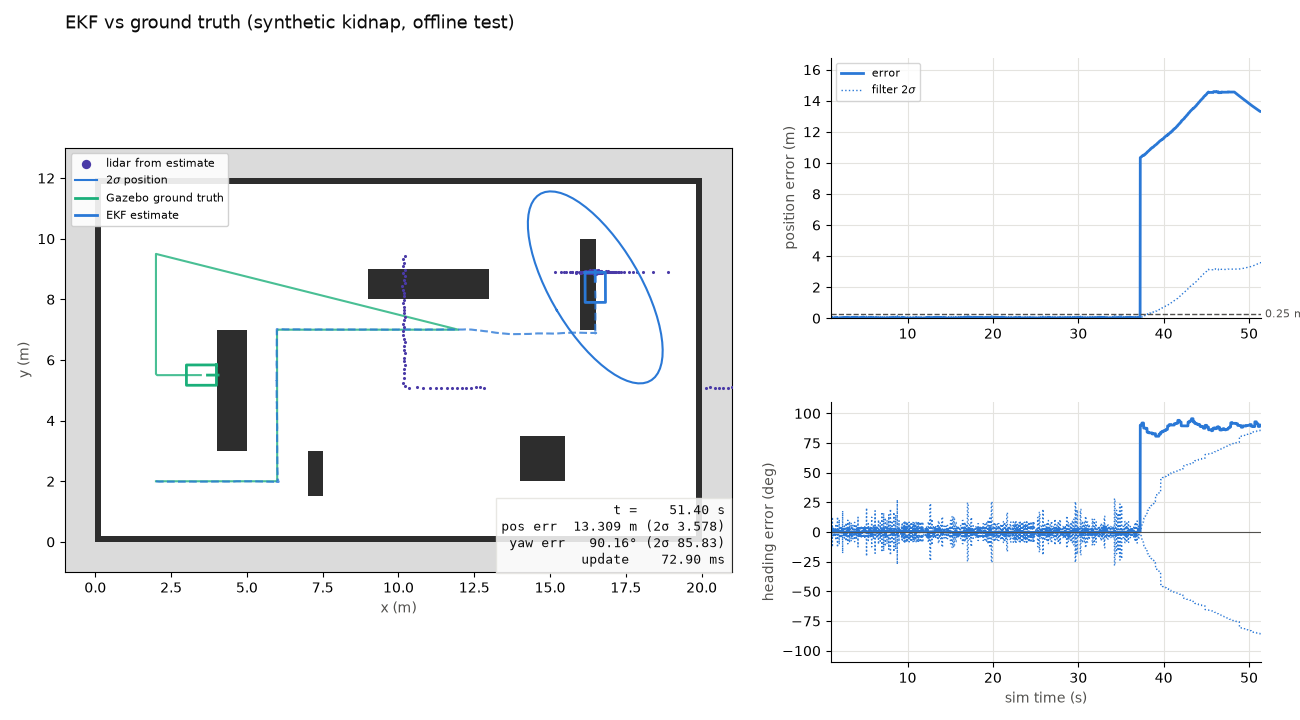
\includegraphics[width=\linewidth]{synthetic_kidnap_ekf.png}
\caption{EKF on the offline synthetic kidnap test. Left: map, ground truth (green), EKF estimate and $2\sigma$ ellipse (blue), and the LIDAR scan projected from the estimate. Right: position and heading error against the filter's own $2\sigma$ bound. After the teleport at about 37~s the error jumps above 10~m and never returns; the covariance grows but the single Gaussian cannot jump to the true pose.}
\label{fig:prelim-kidnap-ekf}
\end{figure}

\begin{figure}[H]
\centering
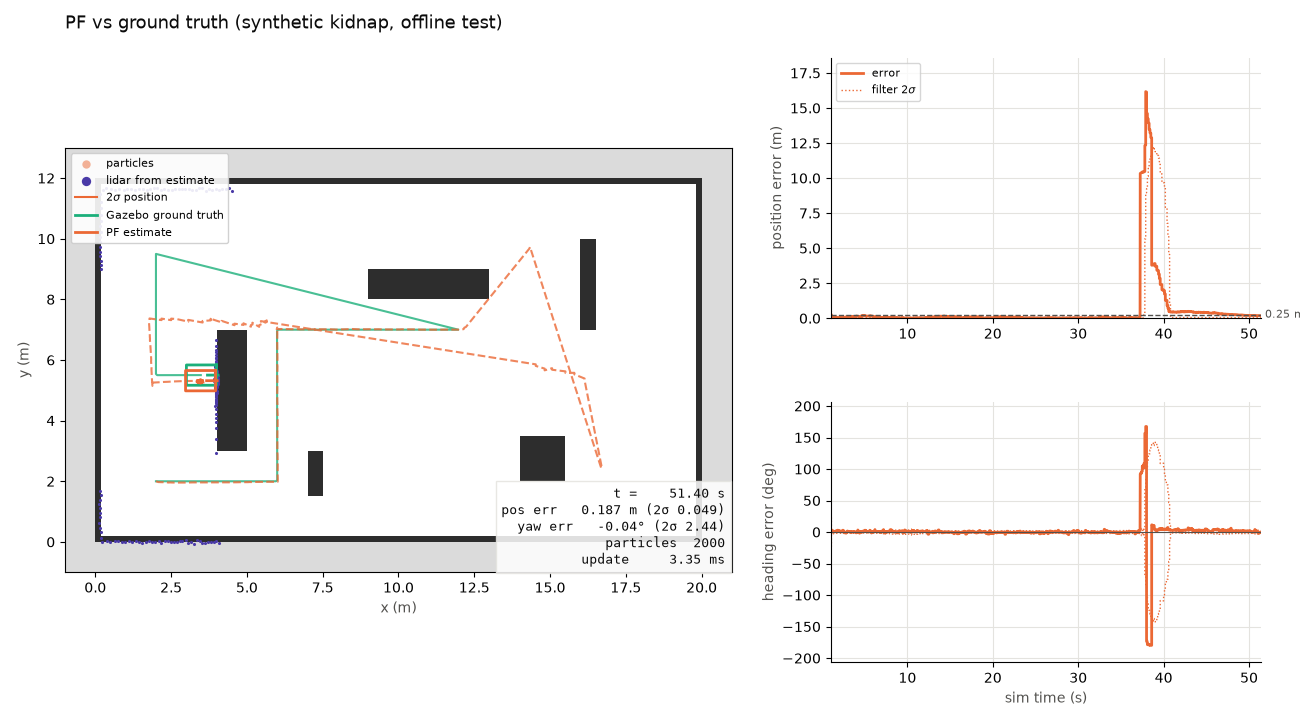
\includegraphics[width=\linewidth]{synthetic_kidnap_pf.png}
\caption{PF on the same offline synthetic kidnap test ($N = 2000$). The error spikes above 15~m at the teleport and falls back under the 0.25~m threshold within about 11~s as injected particles find the true pose.}
\label{fig:prelim-kidnap-pf}
\end{figure}

\begin{figure}[H]
\centering
\begin{subfigure}{0.49\linewidth}
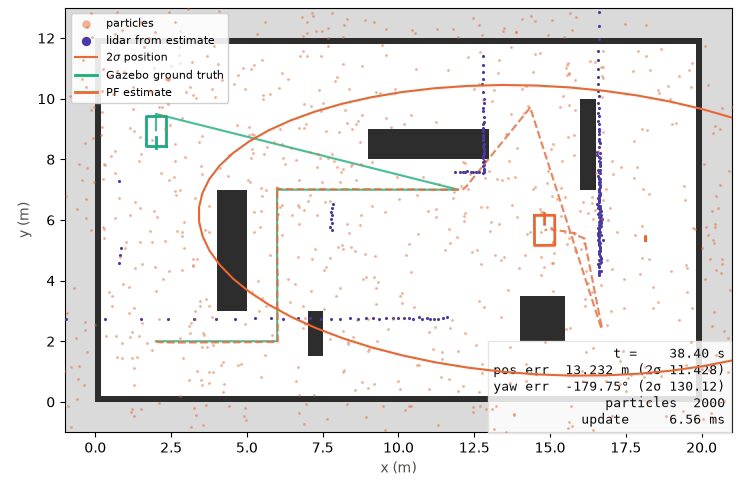
\includegraphics[width=\linewidth]{synthetic_kidnap_pf_dispersed.png}
\caption{$t = 38.4$~s: particles spread across the map, broad $2\sigma$ ellipse.}
\end{subfigure}
\hfill
\begin{subfigure}{0.49\linewidth}
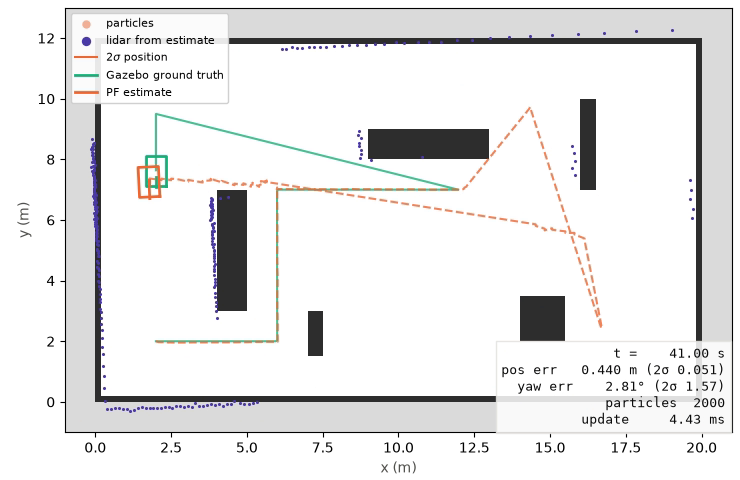
\includegraphics[width=\linewidth]{synthetic_kidnap_pf_reconverging.png}
\caption{$t = 41.0$~s: cloud collapsed near the true pose (0.44~m error).}
\end{subfigure}
\caption{Stills from the PF live view during kidnap recovery (offline synthetic), showing the intermediate posterior. The full recording is \texttt{localization-viz/synthetic\_kidnap\_pf.mp4} in the project files; Gazebo recordings are written to \texttt{results/} by the \texttt{localization\_sim} launch file.}
\label{fig:prelim-kidnap-stills}
\end{figure}

\paragraph{Still to come.}
The 20-seed runs of the nominal, kidnap, and global-localization scenarios and the one-factor-at-a-time sweep over $N$, $k$ and $\sigma_r$ are in progress; their mean $\pm$ 95\% CI tables and recovery-rate intervals will replace the single-seed tables above, and Gazebo stills of both filters will replace the synthetic figures.

\section{Conclusion}\label{Conclusion}
The final section will synthesize the experimental results to definitively answer whether the primary hypothesis holds true: that the Particle Filter recovers in both adversarial scenarios where the EKF does not, and that the EKF matches or exceeds nominal-route accuracy at lower per-step compute time. It will discuss the practical implications of these findings for the robotic system's downstream waypoint controller and planning pipeline. Lastly, it will propose future work, such as mitigating the noted implementation asymmetry or extending the evaluation to dynamic obstacles within the factory.

\section*{Acknowledgments}\label{sec:Acknowledgments}
Anthropic's Claude was used to review this outline against the course rubric and the instructor's feedback on the proposal, to draft revisions to it, and to summarize the preliminary trial results and extract figure stills from the filter visualizations. The localization nodes, evaluation tooling and simulation runs reported here were also developed with Claude's assistance.

\bibliography{ref}

\end{document}